%%%%%%%%%%%%%%%%%%%%%%%%%%%%%%%%%%%%%%%%%
% Thin Sectioned Essay
% LaTeX Template
% Version 1.0 (3/8/13)
%
% This template has been downloaded from:
% http://www.LaTeXTemplates.com
%
% Original Author:
% Nicolas Diaz (nsdiaz@uc.cl) with extensive modifications by:
% Vel (vel@latextemplates.com)
%
% License:
% CC BY-NC-SA 3.0 (http://creativecommons.org/licenses/by-nc-sa/3.0/)
%
%%%%%%%%%%%%%%%%%%%%%%%%%%%%%%%%%%%%%%%%%

%----------------------------------------------------------------------------------------
%	PACKAGES AND OTHER DOCUMENT CONFIGURATIONS
%----------------------------------------------------------------------------------------

\documentclass[a4paper, 11pt]{article} % Font size (can be 10pt, 11pt or 12pt) and paper size (remove a4paper for US letter paper)

\usepackage[protrusion=true,expansion=true]{microtype} % Better typography
\usepackage{graphicx} % Required for including pictures
\usepackage{wrapfig} % Allows in-line images
\usepackage{hyperref}

\usepackage{mathpazo} % Use the Palatino font
\usepackage[T1]{fontenc} % Required for accented characters
\linespread{1.05} % Change line spacing here, Palatino benefits from a slight increase by default

\makeatletter
\renewcommand\@biblabel[1]{\textbf{#1.}} % Change the square brackets for each bibliography item from '[1]' to '1.'
\renewcommand{\@listI}{\itemsep=0pt} % Reduce the space between items in the itemize and enumerate environments and the bibliography

\renewcommand{\maketitle}{ % Customize the title - do not edit title and author name here, see the TITLE block below
\begin{flushright} % Right align
{\LARGE\@title} % Increase the font size of the title

\vspace{50pt} % Some vertical space between the title and author name

{\large\@author} % Author name
\\\@date % Date

\vspace{40pt} % Some vertical space between the author block and abstract
\end{flushright}
}

%----------------------------------------------------------------------------------------
%	TITLE
%----------------------------------------------------------------------------------------

\title{\textbf{No Country for Old Web}\\ % Title
Keeping web crawl data updated} % Subtitle

\author{\textsc{Primal Pappachan} % Author
\\{\textit{University of Maryland, Baltimore County}}} % Institution

\date{\today} % Date

%----------------------------------------------------------------------------------------

\begin{document}

\maketitle % Print the title section

%----------------------------------------------------------------------------------------
%	ABSTRACT AND KEYWORDS
%----------------------------------------------------------------------------------------

%\renewcommand{\abstractname}{Summary} % Uncomment to change the name of the abstract to something else

\begin{abstract}

Search engines are one of the most used web applications today. Outlines some of the challenges and goes deep into the the topic of refresh policies related to web crawling. Surveys existing techniques to solve the problem and also verifies how much of challenges mentioned in seminal papers were covered and presents new challenges to be tackled in this domain.

\end{abstract}

\hspace*{3,6mm}\textit{Keywords:} webcrawling , refresh policies , search engine , revisiting policies % Keywords

\vspace{30pt} % Some vertical space between the abstract and first section

%----------------------------------------------------------------------------------------
%	ESSAY BODY
%----------------------------------------------------------------------------------------

\section*{Introduction}

For many of us a search engine is the starting point of the Internet. We browse the web using Google, Bing, DuckDuckGo or any other search engine to find what we are looking for. In a nutshell, an user interacts with search engine by entering some keywords as a query and receive web pages that contain the keyword and ranked according to relevancy. \\

This is an oversimplified explaination of how the search engine works. The size of web and the frequency at which it changes makes it much more challenging than a simple information retrieval problem. To add some perspective to the problem at hand, 20 million pages were indexed by AltaVista in 1995 when most of the seminal papers related to this topic were written. Fast-forwarding to 2008, 1 trillion URLs were known by Google and Yahoo. Each of web pages contained 10 - 100 KB of textual content and roughly has 100 links per page. \cite{stats2008st} \\ 

Before going into the details of Web Crawling, it is important to understand how a search engine is assembled together. Figure 1 below the schema of a search engine from the works of \cite{arasu2001searching}. As seen in the figure, a search engine relies on a \textit{crawler} which browses the Web on it's behalf. Starting from a set of URLs, this module follows the links and retrieve pages from the Web into a page repository until a stop criterion is met. Crawling operations will be explained in more detail in the following section. \\

\begin{figure} % Inline image example
\begin{center}
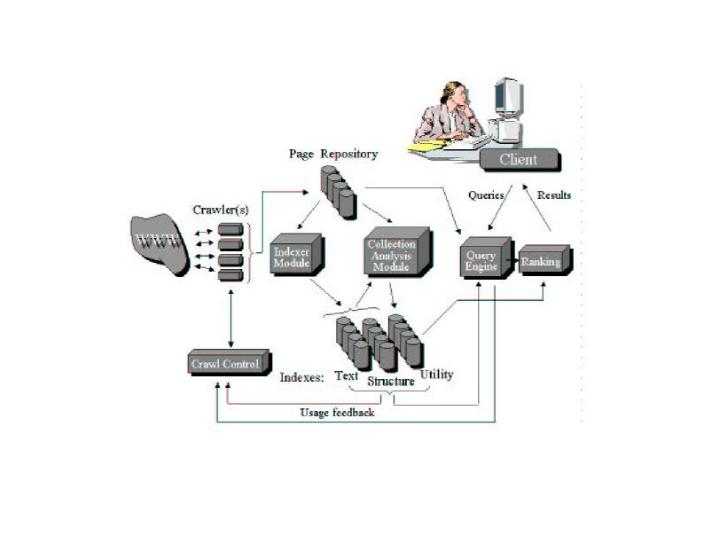
\includegraphics[width=1\textwidth]{searchengine.jpg}
\end{center}
\caption{Searching the web}
\end{figure}

The indexer module builds an index by extracting tokens from the pages in the repository. It generates a look up table where words act as keys and the URLs that point to the page they occur in are values. The collection analysis module is responsible for creating various types of utility indexes which provides access to pages with specific structure and content (contains some number of images) \cite{arasu2001searching}. Query engine deals with user requests and uses the indexes to retrieve the URLs of relevant pages from the repository. Ranking module does the task of sorting results so that results near the top are most likely to be of interest to the user. \\

In rest of the paper, we describe in more detail the web crawling aspect of the search engine. This paper serves as an Introduction to the challenges associated with keeping web crawl updated and some interesting techniques that have been developed over the years. \\


\section{Web Crawling}

As mentioned earlier web crawling is a small program that browses the Web on the behalf of search engine. They are given a starting set of urls (seed / initial urls) whose pages they retrieve from the Web. The crawler also extracts the urls appearing in the retrieved pages and adds it to a queue (to visit urls). The retrieved pages are added to a repository and the crawler goes onto visit urls from the to visit queue. \cite{baeza1999modern} 

\begin{figure}[h] % Inline image example
\begin{center}
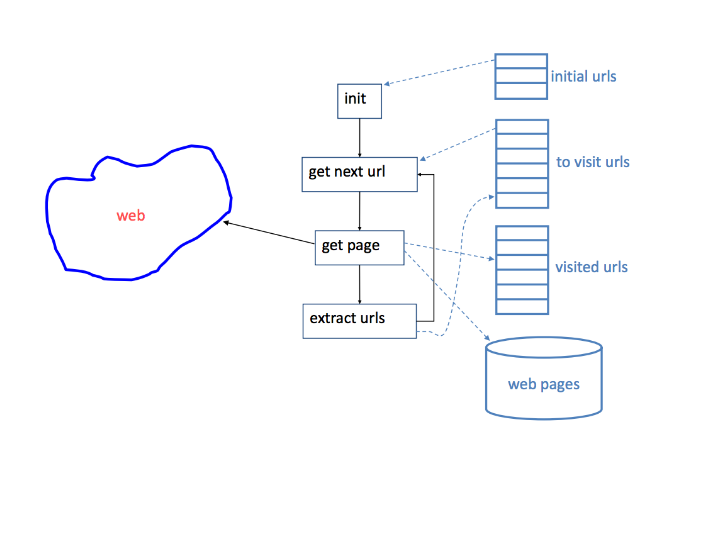
\includegraphics[width=1\textwidth]{webcrawling.png}
\end{center}
\caption{What is a web crawler?}
\end{figure}

\subsection{Crawling Challenges}

As mentioned earlier, the Web is enormous and changing frequently. Therefore web crawling comes with its unique set of challenges as outlined by \cite{arasu2001searching}.

\begin{enumerate}

\item What pages should the crawler download?

Since the Web is so large, a crawler can only download a small portion of the Internet. It has to carefully select important pages for crawling by prioritizing the urls in to visit queue properly so that portion of the Internet it has visited is significant.

\item How should the crawler refresh pages? 

One of the unique challenges of Information retrieval in the Web is how often the web pages change. Therefore a crawler has to revisit the pages and refresh their contents in the repository so that the local copy of Web maintained by the crawler is not out-of-date with respect to the remote one. In the next section we will be explaining in more detail about challenges involved in maintaining the \textit{freshness} of the collection and techniques to solve them.

\item How to be unobstrusive on the web servers being visited?

When a crawler is working, it consumes resources belonging to other organizations such as disk, CPU resources and network bandwidth. Therefore the crawler should minimize the impact on other web servers so that the administrators of those website would not complain.

\item How to parallize the crawling the process? 

Web crawling is a time consuming process and steps should be taken to reduce this time by running the crawler on multiple machines and parallelizing the downloads of pages. Additionally, these parallel crawlers should be coordinated properly so that they do not interfere with each other's working and does not violate the crawling policy. Coordination can incur communication overhead and therefore limits the number of simultaneous crawlers possible. 

\end{enumerate}

\subsection{Crawler Objective}

According to Coffman et. al \cite{coffman1997optimal}, one of the main objectives of a crawler is to minimize the fraction of time pages remain outdated. This can be split into two different objectives based on two different metrics. 

\begin{itemize}
\item Keep the average freshness of pages high
\item Keep the average age of pages low
\end{itemize}

The cost functions age and freshness are defined as follows by \cite{cho2000synchronizing}.

\begin{figure}[h] % Inline image example
\begin{center}
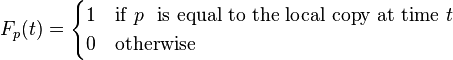
\includegraphics[width=1\textwidth]{freshness.png}
\end{center}
\caption{Freshness of a page p at time t}
\end{figure}

Freshness represents the fraction of up-to-date pages in the repository. When all pages in the local repository are synchronized with that of the remote repository, freshness is 1. On the other hand, age is a measure of how old the downloaded copies of web pages are. These two metrics are related and similar.

\begin{figure}[h] % Inline image example
\begin{center}
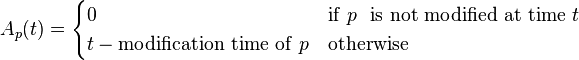
\includegraphics[width=1\textwidth]{age.png}
\end{center}
\caption{Age of a page p at time t}
\end{figure}

\subsection{Crawler Design Issues}

In their seminal paper in 1999 Cho et. al \cite{cho1999evolution} describes about various crawler design issues and their possible trade offs. They identified two types of crawlers with constrasting features so as to tackle the web crawling challenges earlier mentioned.

The first of these is a periodic crawler and their features are

\begin{itemize}
\item Batch mode - periodically updates the entire collection in a single crawl
\item Shadowing - new set of pages are collected and stored in a separate space and replaces the current collection at the end of the crawl
\item Fixed frequency - revisits all pages at same frequency irrespective of how ofthen they change
\end{itemize} 

Secondly, we have the incremental crawler with a constrasting set of features with that of a periodic crawler.

\begin{itemize}

\item Steady mode - crawler runs continously and incrementally updates the collection
\item In place - updates the web pages in place by replacing old version with new version when it is downloaded
\item Variable frequency - optimizes revisits based on how frequently they change 

\end{itemize}

\begin{table}
\begin{tabular}{|c|c|c|}
\hline 
\textbf{Periodic Crawler} & Easy to implement & High availability \\ 
\hline 
\textbf{Incremental Crawler }& High freshness & Minimal load on network and servers \\ 
\hline
\end{tabular} 
\caption{Periodic versus incremental} 
\end{table}

Architecture of an incremental crawler add the diagram and some explanation

\section{Revisiting policies}

\cite{cho2003effective}

\subsection{Uniform Policy}

\subsection{Proportional Policy}

\subsection{Optimal Policy}

\section{Future work}

\subsection{Proposed}

\subsection{Current status}

\subsection{What still needs to be done}

\section{Conclusion}

\section*{Appendix}

Presentation Link: \url{http://bit.ly/primal676}


%----------------------------------------------------------------------------------------
%	BIBLIOGRAPHY
%----------------------------------------------------------------------------------------

\bibliographystyle{unsrt}

\bibliography{references}

%----------------------------------------------------------------------------------------

\end{document}